\section{System initialization}
We are now ready to initialize the MD system. We assume that we will simulate an system with volume 
\begin{align}
	V=L_xL_yL_z,
\end{align}
where $L_i$ is the system size in the $i$th dimension. The system contains $N$ argon atoms and is performed on
\begin{align}
	P = P_xP_yP_z 
\end{align}
processors, $P_i$ being the number of processors in the $i$th dimension. Each processor controls a volume 
\begin{align}
	V_p = l_xl_yl_z,
\end{align}
where $l_i = L_i/P_i$ is the node length. The origin of processor $(p_x, p_y, p_z)$ is given as
\begin{align}
 	\vec p_\text{origin}(p_x, p_y, p_z) = p_xl_x\hat i + p_yl_y\hat j + p_zl_z \hat k.
\end{align}
The initialization process consists of creating the atoms, place them at some position and give them velocities according to the Maxwell-Boltzmann distribution (equation \eqref{eq:maxwell_boltzmann_vector_probability}). We will initially place the atoms on an face-centered cubic lattice (FCC lattice).
\subsection{FCC lattice}
The FCC lattice is a lattice structure where we place atoms on all 8 corners of a cube in addition to all the faces, hence the name. In figure \ref{fig:md_fcc} we see how the atoms are placed on the FCC lattice.
\begin{figure}[h!]
\begin{center}
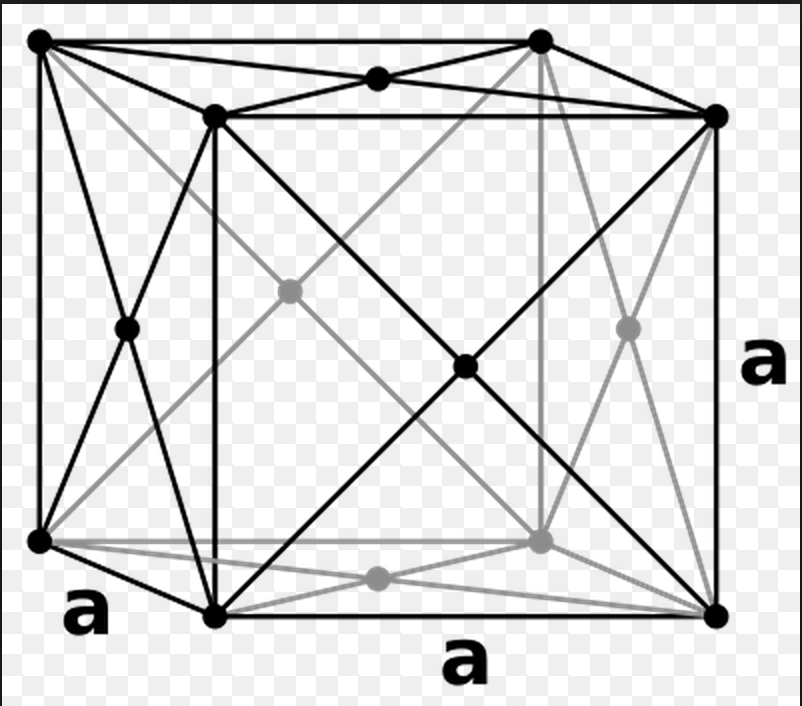
\includegraphics[width=0.7\textwidth, trim=0cm 0cm 0cm 0cm, clip]{MD/figures/fcc.png}
\end{center}
\caption{The face-centered cubic lattice. There are atoms on all eight corners of a cube, in addition to the six faces. The length $a$ is called the lattice constant. (Image from \url{http://en.wikipedia.org/wiki/File:Lattice_face_centered_cubic.svg}, accessed 19 March, 2014.)}
\label{fig:md_fcc}
\end{figure}
An FCC lattice can be constructed from a unit cell consisting of four atoms with local positions (relative to the origin of the unit cell)
\begin{align}
	\vec r_1 &= 0\ihat + 0 \jhat + 0 \khat\\
	\vec r_2 &= \frac{a}{2}\ihat + \frac{a}{2} \jhat + 0 \khat\\
	\vec r_3 &= 0\ihat + \frac{a}{2} \jhat + \frac{a}{2} \khat\\
	\vec r_4 &= \frac{a}{2}\ihat + 0 \jhat + \frac{a}{2} \khat,
\end{align}
where $a$ is the lattice constant, the length of the unit cell. By adding several such unit cells, each with origin determined by the unit cell coordinate $(m,n,l)$
\begin{align}
	\vec r_\text{unit cell} = ma\ihat + na\jhat + la\khat,
\end{align}
we can create a system of arbitrary size. Each atom is assigned a random velocity according to the Maxwell-Boltzmann distribution. The total number of atoms in the system is based on how many unit cells we create. If we label the number of unit cells \textit{per processor} in the $i$th dimension $N_c^{(i)}$, the total number of unit cells is
\begin{align}
	N_c = N_c^{(x)}N_c^{(y)}N_c^{(z)} P,
\end{align}
which gives the total number of atoms (each unit cell contains 4 atoms)
\begin{align}
	N = 4N_c.
\end{align}
The system size is then
\begin{align}
	L_x &= aN_c^{(x)}P_x\\
	L_y &= aN_c^{(y)}P_y\\
	L_z &= aN_c^{(z)}P_z,
\end{align}
yielding a total volume $V = a^3N_c$. In listing \ref{lst:md_fcc_lattice}, we have shown how this is implemented in C{}\verb!++!.
\begin{lstlisting}[caption=Code example showing how to create an FCC lattice on one of the processors., label=lst:md_fcc_lattice]
void create_fcc_lattice() {
    double xCell[4] = {0, 0.5, 0.5, 0};
    double yCell[4] = {0, 0.5, 0, 0.5};
    double zCell[4] = {0, 0, 0.5, 0.5};

    int index = 0;
    double velocity_standard_deviation = sqrt(boltzmann_constant*temperature/mass);
    for(int x = 0; x < unit_cells_per_cpu_x; x++) {
        for(int y = 0; y < unit_cells_per_cpu_y; y++) {
            for(int z = 0; z < unit_cells_per_cpu_z; z++) {
                // Loop over the 4 atoms in this unit cell
                for(int k = 0; k < 4; k++) {
                    positions.at(index).x = (x+xCell[k]) * FCC_a;
                    positions.at(index).y = (y+yCell[k]) * FCC_a;
                    positions.at(index).z = (z+zCell[k]) * FCC_a;
                    velocities.at(index).x = rnd.nextGauss()*velocity_standard_deviation;
                    velocities.at(index).y = rnd.nextGauss()*velocity_standard_deviation;
                    velocities.at(index).z = rnd.nextGauss()*velocity_standard_deviation;
                    index++; // Increase atom counter
                }
            }
        }
    }
}
\end{lstlisting}
This is the whole initialization process. The atoms are where they should be, they have a statistically correct velocity and we are ready to integrate forward in time.